% Section content template for individual Educative lessons
% This file contains the actual content for a specific section
% Generated from Educative API section content

% Section: Sequence Diagram for the Library Management System
% Section ID: 4655341294059520
% Section Slug: sequence-diagram-for-the-library-management-system
% Generated: 2025-12-11T15:13:24.932748

Sequence diagrams help visualize the flow of interactions between different entities and objects in the system, step by step. This lesson will illustrate the main interactions in lending and returning a book within the library management system. Understanding these workflows is essential for modeling object responsibilities and collaborations.
\\
For this lesson, we will focus on the following two scenarios:

\begin{itemize}
\item
\protect\phantomsection\label{lEigJCxUCZa-Q2wnHRRI3}
\textbf{Issuing (Lending) a book:} The process through which a member requests to borrow a book from the library.
\item
\protect\phantomsection\label{OmgU-1Sga5MYpMvnLj9dl}
\textbf{Returning a book:} The process for when a member returns a borrowed book to the library.
\end{itemize}

\subsection{Issuing (Lending) a book}\label{mMU7SolVaBdffq7vaUkCT}
\\
The sequence diagram for issuing a book involves the following participants:

\begin{itemize}
\item
\protect\phantomsection\label{35IHkTCdUBR1yiRuiT0BH}
\textbf{Actors:} \texttt{Member} and \texttt{Librarian}
\item
\protect\phantomsection\label{nmh1-Lx73rQiA8PMRecrf}
\textbf{Objects:} \texttt{Book} and \texttt{BookItem}
\end{itemize}
\\
The typical workflow is as follows:

\begin{enumerate}
\item
\protect\phantomsection\label{51Mv7obssQEgVjF7AovsK}
\textbf{Member requests to issue a book:}

\begin{enumerate}
\item
The member initiates the process by asking the librarian to issue a specific book.
\end{enumerate}
\item
\protect\phantomsection\label{eT3k-2adttgYumZ1fW47E}
\textbf{Librarian checks the member's quota:}

\begin{enumerate}
\item
The librarian verifies whether the member has reached their maximum allowed number of borrowed books.

\begin{enumerate}
\item
If the quota is reached:

\begin{enumerate}
\item
The librarian informs the member that no more books can be issued now.
\end{enumerate}
\item
If quota is available:

\begin{enumerate}
\item
The librarian proceeds to check the status of the requested book.
\end{enumerate}
\end{enumerate}
\end{enumerate}
\item
\protect\phantomsection\label{yYs-R_eM8-y_ANmumQ-8H}
\textbf{The librarian checks the book's status:}

\begin{enumerate}
\item
If the book is \emph{available}:

\begin{enumerate}
\item
The librarian issues the book to the member, updating lending records accordingly.
\end{enumerate}
\item
If the book is \emph{reserved} (by another member):

\begin{enumerate}
\item
The librarian informs the requesting member that the book cannot be issued.
\end{enumerate}
\end{enumerate}
\end{enumerate}
\\
The sequence diagram below visualizes these interactions, clearly showing the flow of requests, validations, and responses between the member, librarian, and book entities.

\begin{figure}[htbp]
 \centering
 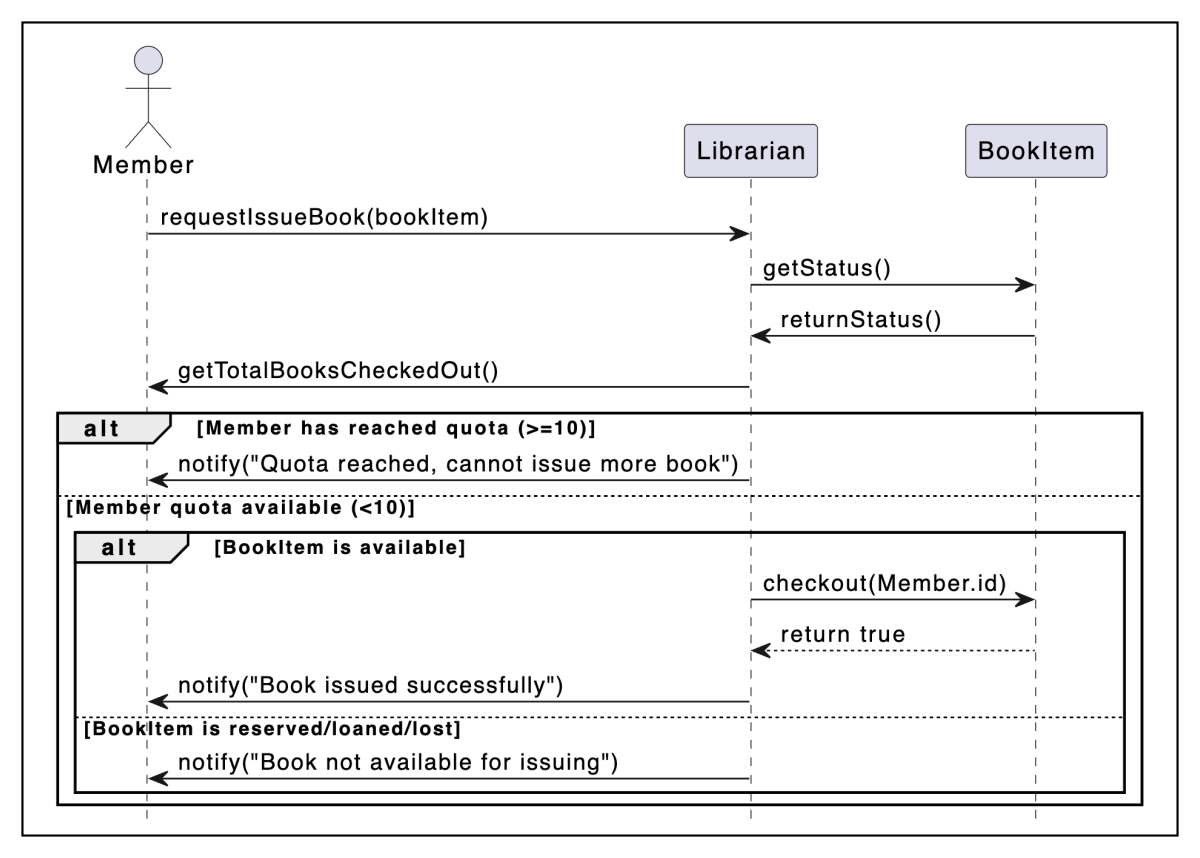
\includegraphics[width=0.5\textwidth]{Images/chapter_9/section_4655341294059520/4818255129477120.png}
 \caption{The sequence diagram for issuing a book}
\end{figure}

\begin{center}\rule{0.5\linewidth}{0.5pt}\end{center}

\subsection{Sequence challenge: Return a book}\label{sg-z_TAJHHvo52e9BsTw9}
\\
You will complete a sequence diagram for returning a book to the library. The diagram below demonstrates a skeleton for this process.

\begin{figure}[htbp]
 \centering
 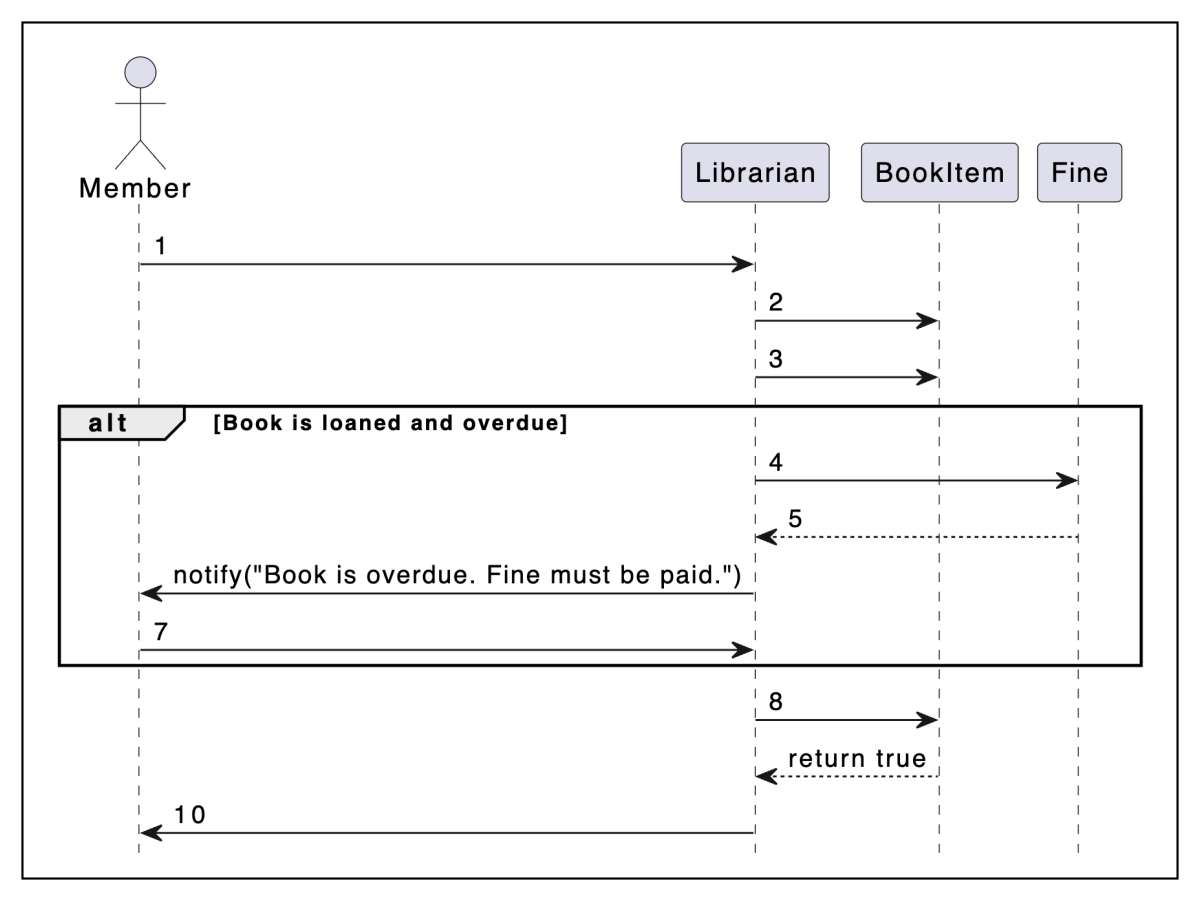
\includegraphics[width=0.5\textwidth]{Images/chapter_9/section_4655341294059520/5170108849586176.png}
 \caption{The sequence diagram for returning a book}
\end{figure}

Notice that the arrows in the above diagram are numbered from 1 to 13. Below are the messages between the actor(s) and object(s). Can you rearrange the messages below in the correct order sequence they should appear in the sequence diagram's skeleton above?
\begin{quote}
\textbf{Note:} If you're stuck, click the ``Show Solution'' button.
\end{quote}

Alternatively, you can also click the ``Show complete diagram'' button below to view the complete sequence diagram of the return book sequence.

We will create activity diagrams for our library management system in the next lesson.

% End of section content